\section{Upload Evaluation}\label{sec:uploadeval}
We evaluate the upload path with real CIFAR-10 TRAIN updates, loopback HTTP, SQLite state and the Solidity registry on a local EVM development chain. Activities with two clients over two rounds and five clients over three rounds share the same measurement boundaries and recovery protocol. This pairing tests the transition from a compact encoded update to a recoverable contribution in the shared model.

\subsection{Compact messages retain their bound context}
For the 136,874-parameter model, uniform3 produces 54,067 B including block scales and the codec header, compared with 547,560 B for the dense message profile. The authenticated envelope adds 341 B, giving 54,408 B per fresh upload. The two activities carry 217,632 B across four uploads and 816,120 B across fifteen uploads; the unchanged message size keeps the context cost explicit as the activity grows.

Table~\ref{tab:chaincost} separates message bytes, registration gas and verification work. The codec reduces the dense upload profile by 90.13\%, while the authenticated message occupies 9.94\% of that dense profile. Registration calldata measures 356 B per transaction, and signed transactions occupy 472--473 B in the five-client run. Keeping application messages and ledger transactions as separate quantities exposes the cost of anchoring alongside the compression saving.
\begin{table}[!htb]\centering\small
\caption{Anchoring preserves the 54,408 B application message as the activity grows. Registration gas excludes contract deployment; receipt verification measures local authentication and bound chain fields.}\label{tab:chaincost}
\setlength{\tabcolsep}{5pt}
\begin{tabular}{lrr}\toprule
Metric & $2\times2$ & $5\times3$\\\midrule
Fresh uploads & 4 & 15\\
Codec payload / upload (B) & 54,067 & 54,067\\
Authenticated message / upload (B) & 54,408 & 54,408\\
Total fresh message bytes & 217,632 & 816,120\\
Registration gas, total & 1,140,380 & 4,229,478\\
Registration gas / upload, mean & 285,095.0 & 281,965.2\\
Deployment gas, once & 530,120 & 601,869\\
Receipt verification, mean (ms) & 0.457 & 0.380\\
Ledger readback, mean (ms) & 17.912 & 15.573\\\bottomrule
\end{tabular}
\end{table}


\subsection{Fifteen registrations preserve the update trajectory}
The five-client activity uses original clients 0--4 with 450, 159, 1,661, 3,446 and 2,558 TRAIN examples, respectively. Each round runs one local epoch with batch size 64 and learning rate 0.03, yielding 393 gradient evaluations over three rounds. Every computed local update feeds independently encoded direct and protocol paths; FP32 training and coding are followed by FP64 protocol state and deterministic weighted aggregation. After every round, the resulting model and committed residuals match the direct path bit for bit, connecting all fifteen anchored uploads to the same learning trajectory.

The pinned runtime uses Ganache 7.9.2, Solidity 0.8.30 and ethers 6.15.0. Fifteen registrations consume 4,229,478 gas in total, with a mean of 281,965.2 gas per upload; deployment consumes 601,869 gas once. The matched four-registration activity consumes 1,140,380 gas, with a mean of 285,095.0 per upload. Figure~\ref{fig:chaincost} presents these measured configurations with their transaction counts, giving the aggregate cost a concrete workload basis.
\begin{figure}[!htb]\centering
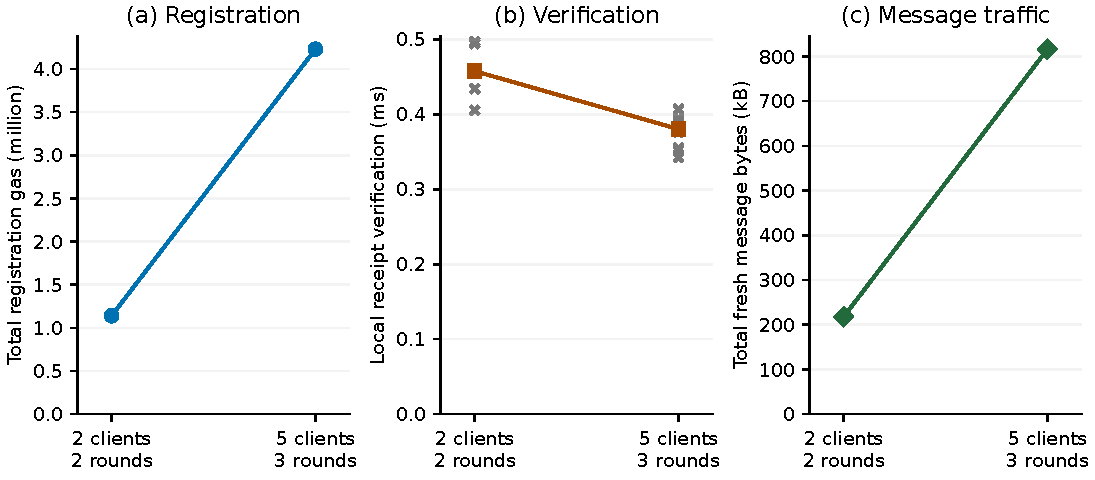
\includegraphics[width=\linewidth]{revision_artifacts/v4_dualtrack/figures/figure4_chain_cost.pdf}
\caption{Measured cost for four and fifteen fresh uploads. Registration gas and message traffic accumulate over the displayed client--round workloads; crosses show individual local receipt-verification times and squares their means.}\label{fig:chaincost}
\end{figure}

Local verification of the first successful commit-path incorporation receipt averages 0.380 ms across fifteen client--round records, compared with 0.457 ms across four records in the smaller activity. This timing includes JSON parsing, HMAC-SM3, freshness, context and embedded chain-field checks; ledger retrieval is timed separately and averages 15.573 ms in the five-client activity. Separating the two measurements identifies the work that authorizes the residual transition after the ledger evidence has arrived.

\subsection{Interrupted responses recover one contribution}
Both activities exercise lost responses after chain registration and after model finalization, reopen service and client databases, and retry the exact pending bytes. Queries recover authenticated incorporated states, while repeated uploads, finalization and residual commits retain the recorded model and generation. Table~\ref{tab:recovery} groups these cases by the interrupted transition, showing how recovery carries the same update through completion.
\begin{table}[!htb]\centering\small
\caption{Recovery resumes the recorded client--round transition. All four classes pass in both measured activities.}\label{tab:recovery}
\setlength{\tabcolsep}{4pt}
\begin{tabular}{p{0.33\linewidth}p{0.48\linewidth}l}\toprule
Injected interruption & Recovered state and action & Result\\\midrule
Reply lost after registration & Read back binding; accept the pending bytes & Pass\\
Reply lost after finalization & Query incorporated record; commit staged residual & Pass\\
Service and database reopen & Restore pending message and persisted model state & Pass\\
Duplicate upload, finalize or commit & Reuse recorded contribution and generation & Pass\\\bottomrule
\end{tabular}
\end{table}


Payload mutations, signed context mismatches, altered receipts and stale challenges are rejected before authorizing the corresponding state transition. In the five-client activity, each round finalizes once and each client generation advances once per round, while recovery adds zero encoding calls, registration requests or model contributions. These outcomes make the authenticated record a bridge between compressed transmission and the state used by subsequent learning.
